\documentclass[compress,12pt,hyperref=unicode]{beamer}
\usetheme{Frankfurt}
\usepackage[utf8]{inputenc}
\usepackage[T1]{fontenc}
\usepackage[english, serbian]{babel}
\usepackage{amsmath}
\usepackage{amsfonts}
\usepackage{amssymb}
\usepackage{graphicx}
\usepackage{textpos}
\usepackage{fancyvrb}
\author{
\texorpdfstring{
\textit{Student}\\Dimitrije Radojević \\ br. ind. 09/0112 \\ \vspace{0.5cm}
\textit{Mentori}\\
Boško Nikolić, PhD\\
Dražen Drašković, MsC}{Dimitrije Radojevic}}
\title{Izrada veb aplikacije za polaganje testova znanja}
\subtitle{\small{Development of web application for taking exams}}
%\setbeamercovered{transparent} 
\setbeamertemplate{navigation symbols}{} 
\graphicspath{{images/}}
\institute{Elektrotehnički fakultet \\ Univerzitet u Beogradu} 
\date{\today}
\AtBeginSection[]
{
  \begin{frame}
    \frametitle{Sadržaj}
    \tableofcontents[currentsection]
  \end{frame}
}
\begin{document}

\begin{frame}[plain]
\titlepage
\begin{textblock*}{2cm}(0.5cm,-3.5cm)

\includegraphics[width=2cm]{etf}
\end{textblock*}
\end{frame}

\section{Uvod}
\begin{frame}
\frametitle{Uvod}
\begin{itemize}
\item Motivacija: pomoć pri učenju gradiva na predmetu Ekspertski sistemi
\item Postojeća rešenja
\begin{itemize}
\item Java aplikacija
\item Mobilna aplikacija
\end{itemize}
\item Predmet rada: izrada veb platforme za polaganje i administraciju testova
\end{itemize}
\end{frame}

\section{Zahtevi za realizacijom}
\begin{frame}
\frametitle{Korisnički zahtevi}
\begin{itemize}
\item Logovanje i registracija
\item Iz perspektive studenta:
\begin{itemize}
\item Pregled testova i istorije polaganja
\item Polaganje testova
\end{itemize}
\item Iz perspektive administratora:
\begin{itemize}
\item Pregled odrađenih testova
\item Izmena ocene testa
\item Dodavanje novih testova
\end{itemize}
\item Unos, transformacija i prikazivanje logičkih izraza (oblast formalne logike, \textit{IR4ES})
\end{itemize}
\end{frame}

\begin{frame}
\frametitle{Korišćene tehnologije}
\begin{itemize}
\item Bekend
\begin{itemize}
\item Pisan u Clojure-u
\item HTTP server: \textit{Ring} + \textit{Compojure} + \textit{Jetty}
\item DB: \textit{PostgreSQL} + \textit{YeSQL}
\item Šabloni: \textit{Hiccup}
\item Parser: \textit{Instaparse}
\end{itemize}
\item Frontend
\begin{itemize}
\item \textit{AngularJS}
\item \textit{Bootstrap} direktive za Angular
\item \textit{KaTeX}
\item aplikacija radi i na mobilnim uređajima
\end{itemize}
\end{itemize}
\end{frame}

\section{Opis rada}
\begin{frame}
\frametitle{Logovanje i registracija}
\begin{center}
\fbox{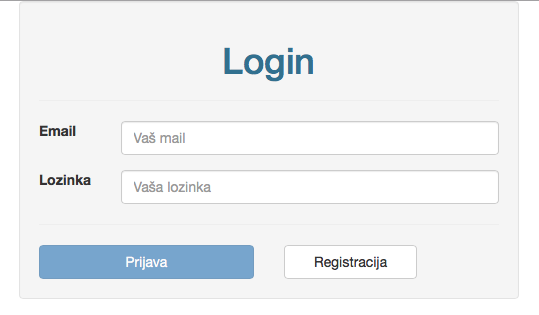
\includegraphics[width=0.45\textwidth]{login}

\includegraphics[width=0.45\textwidth]{register}}
\end{center}
\begin{itemize}
\item Dinamička provera email naloga
\item Nasumična lozinka se šalje na email tokom registracije
\item Kolačići za pamćenje sesije
\end{itemize}
\end{frame}

\begin{frame}
\frametitle{Student: pregled testova}
\fbox{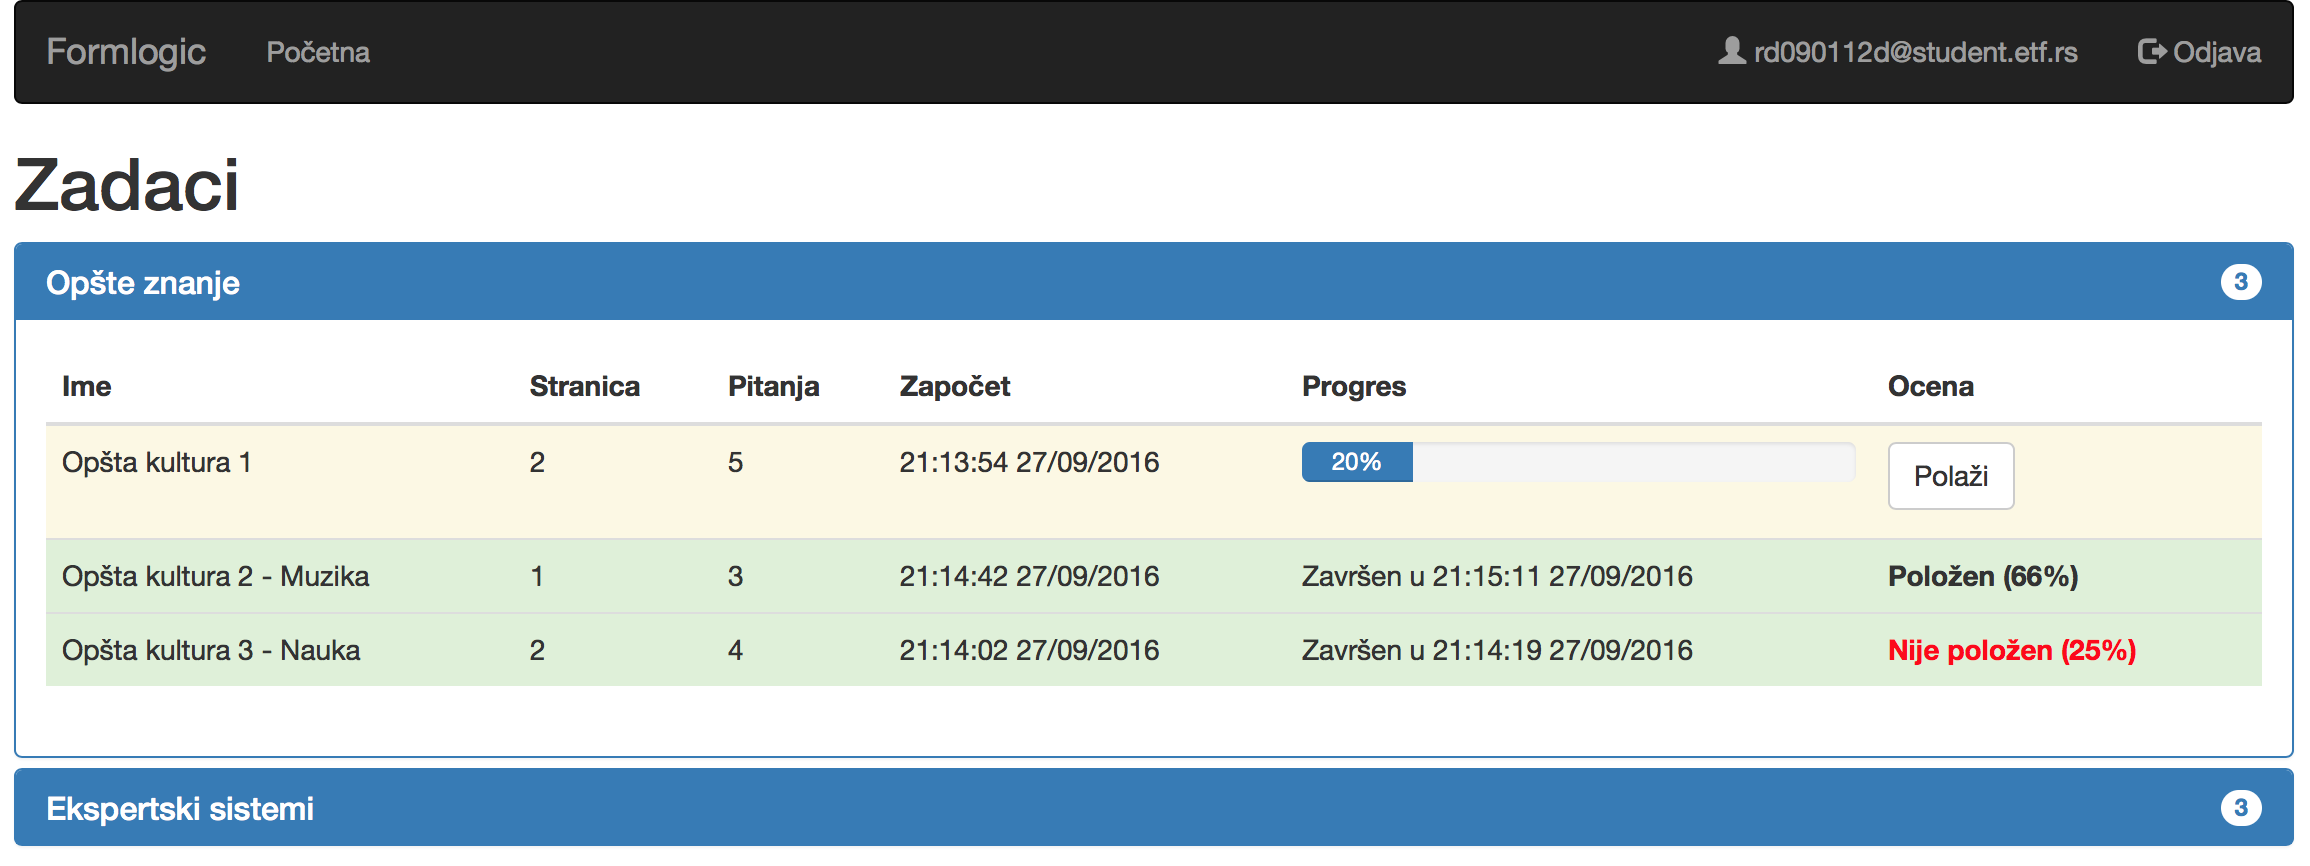
\includegraphics[width=\textwidth]{assignments-collapsed-progress}}
\begin{itemize}
\item Testovi grupisani po kategorijama
\item Istorija polaganja sa datumima polaganja i ocenom
\end{itemize}
\end{frame}

\begin{frame}
\frametitle{Student: polaganje testa}
\begin{itemize}
\item Pitanja grupisana po \emph{stranicama}, sa proizvoljnim brojem pitanja
\item Svaka stranica može imati opcioni panel sa \emph{demonstracijom}
\item Tipovi pitanja:
\begin{enumerate}
\item Više ponuđenih odgovora, jedan tačan
\item Više ponuđenih, više tačnih
\item Odgovor u slobodnoj formi
\end{enumerate}
\item Automatsko ocenjivanje
\end{itemize}
\begin{block}{Demonstracija}
Sadržaj panela sa demonstracijom se specificira u bazi u vidu Clojure koda, koji se evaluira prilikom prikazivanja stranice.
\end{block}
\end{frame}

\begin{frame}
\frametitle{Student: polaganje testa}
\fbox{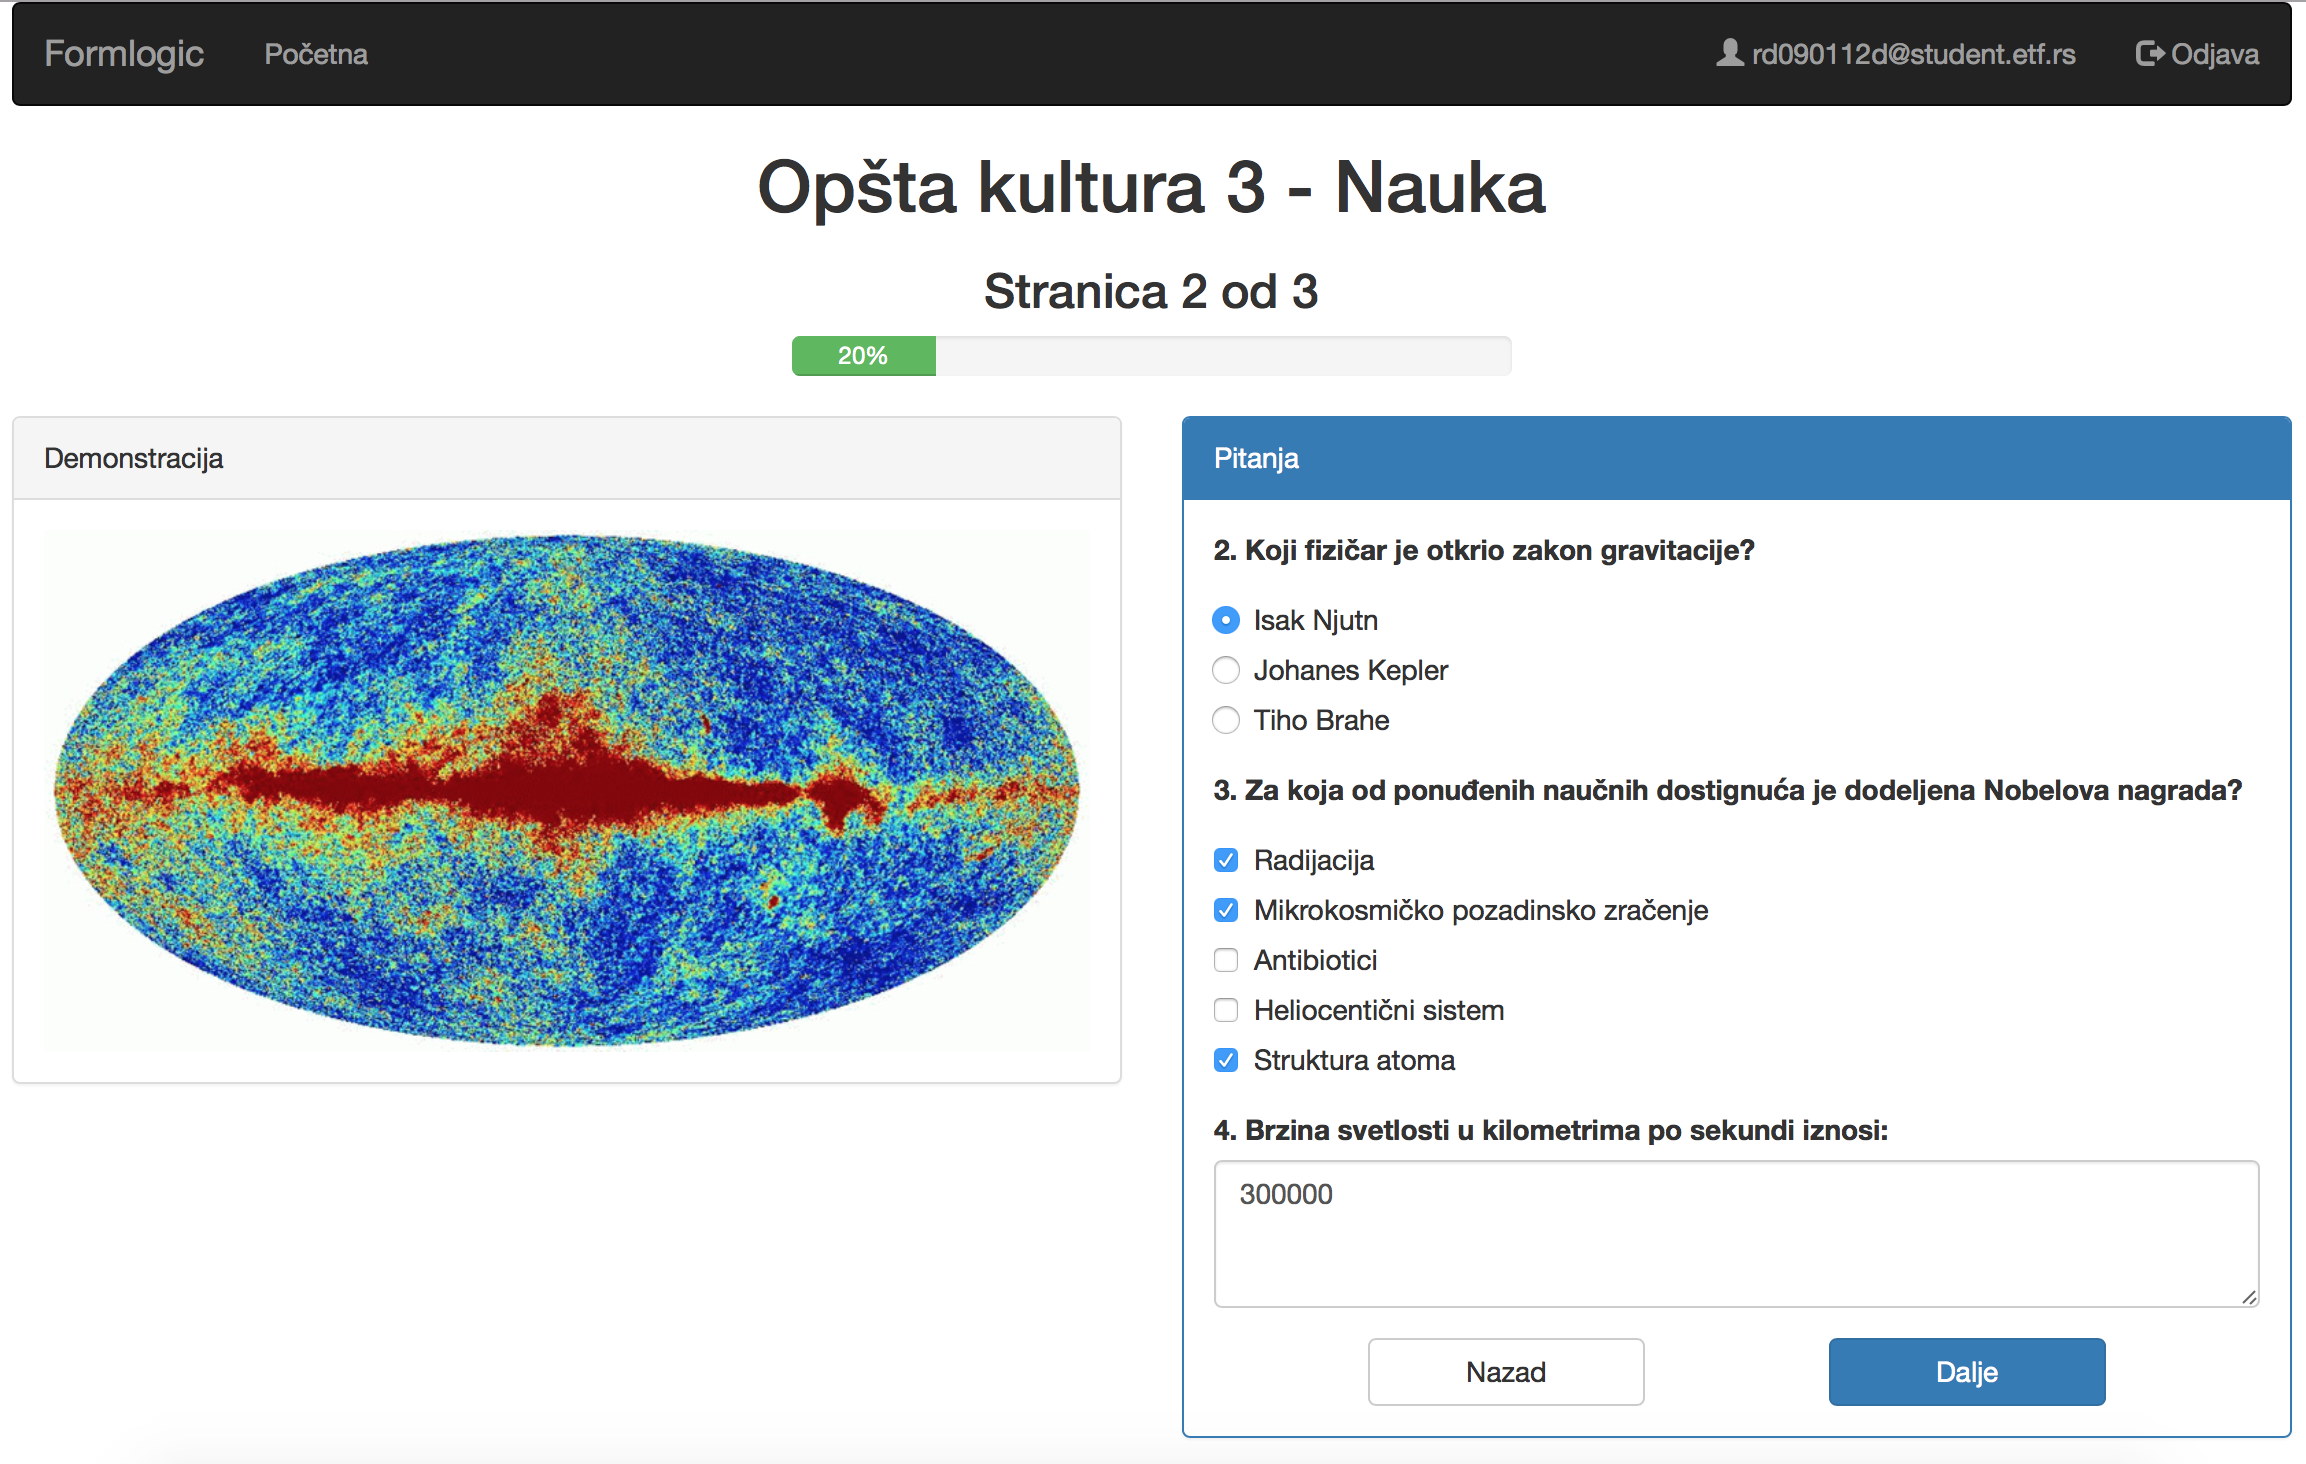
\includegraphics[width=\textwidth]{task}}
\end{frame}

\begin{frame}
\frametitle{Student: polaganje testa}
\begin{columns}
\column{0.5\textwidth}
\centering
\fbox{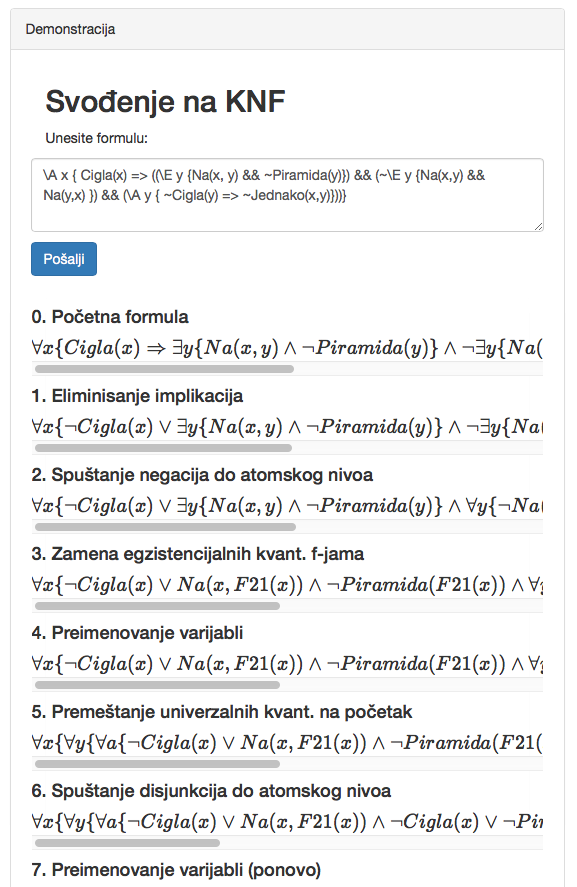
\includegraphics[width=0.8\textwidth]{cnf}}
\column{0.5\textwidth}
Primer panela sa demonstracijom na testu svođenja izraza na KNF formu
\begin{itemize}
\item POST zahtev u pozadini
\item dinamičko prikazivanje rezultata u \LaTeX \space formatu
\item provera greške i detaljan opis
\item ... sve ovo bez prelaska na drugu stranicu
\end{itemize}
\end{columns}
\end{frame}

\begin{frame}
\frametitle{Administrator: pretraga završenih testova}
\fbox{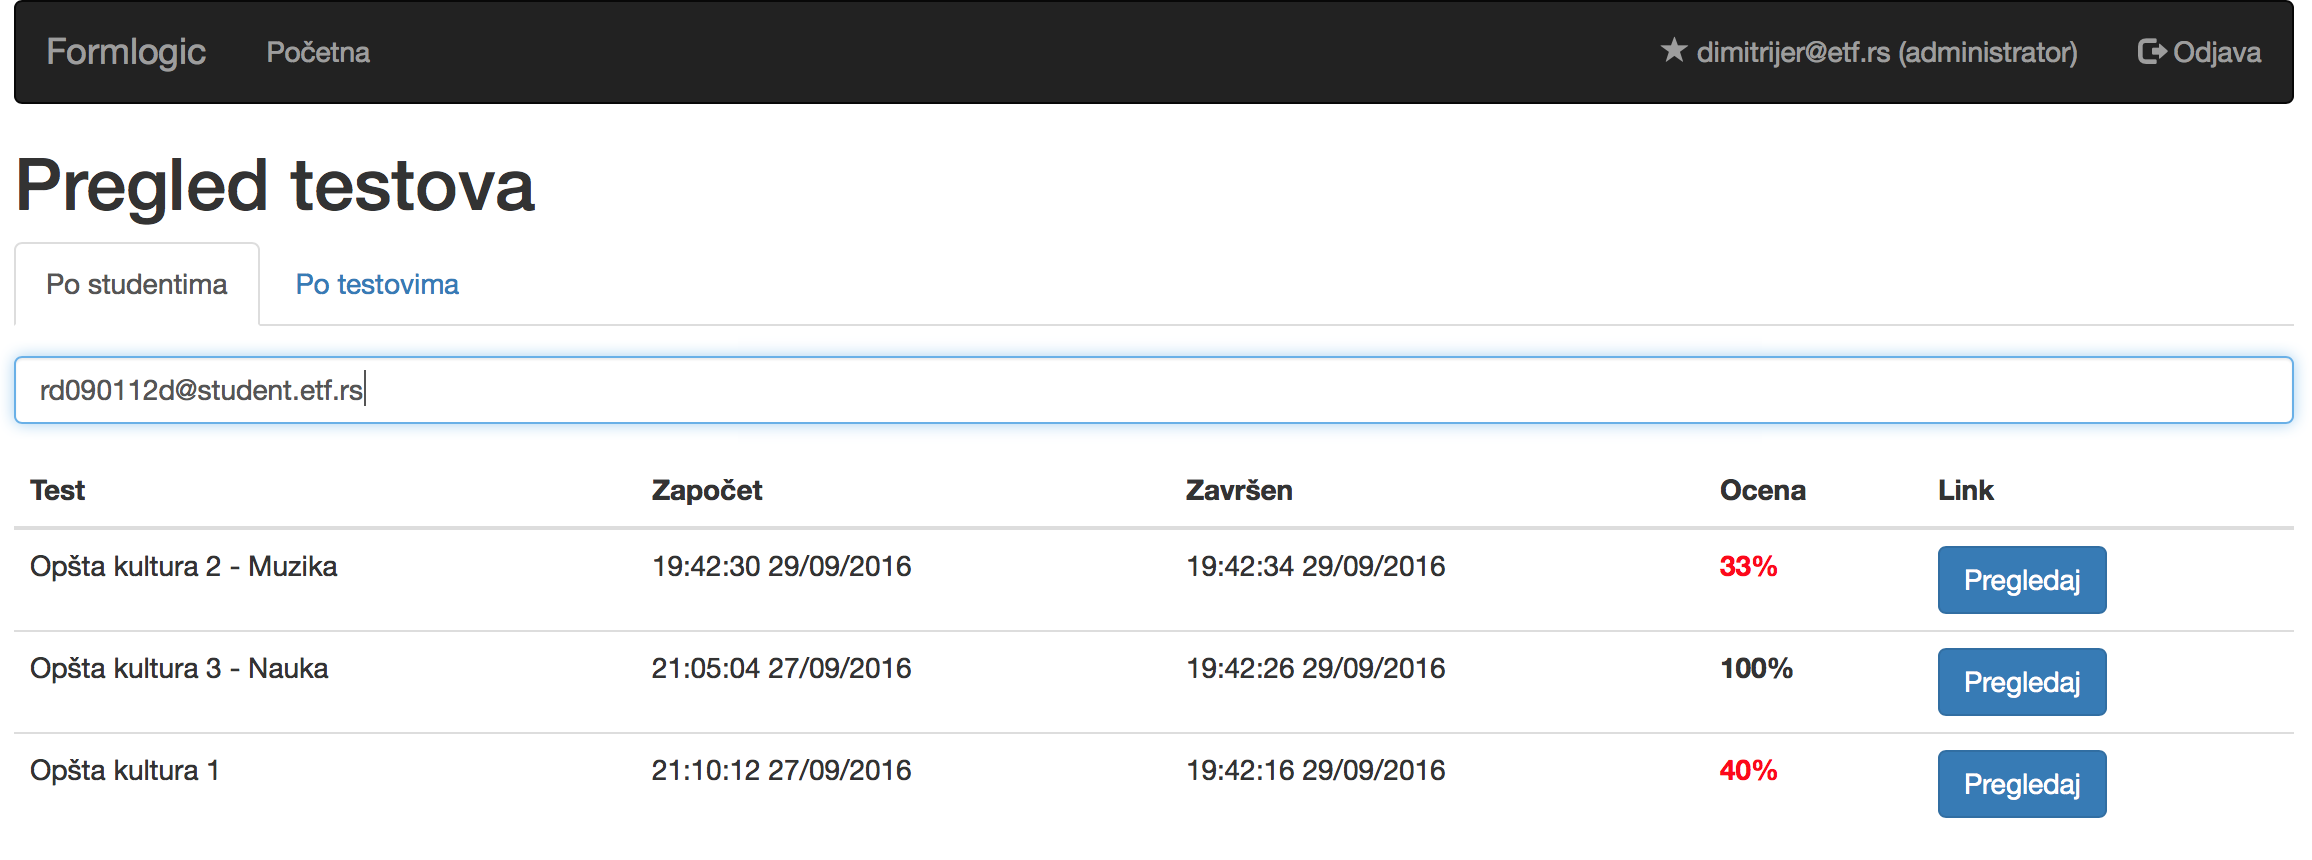
\includegraphics[width=\textwidth]{assignments-admin-student-results}}
\begin{itemize}
\item Pretraga po studentskim nalozima ili po testu
\item Dinamičko sužavanje pretrage (\textit{autocomplete}) prilikom unosa
\end{itemize}
\end{frame}

\begin{frame}
\frametitle{Administrator: pregled testa}
\begin{itemize}
\item Pregled po stranici sa pitanjima
\item Administrator \alert{ne može} menjati odgovore
\item Mogućnost promene automatske ocene po odgovoru
\end{itemize}
\end{frame}

\begin{frame}
\frametitle{Administrator: pregled testa}
\centering
\fbox{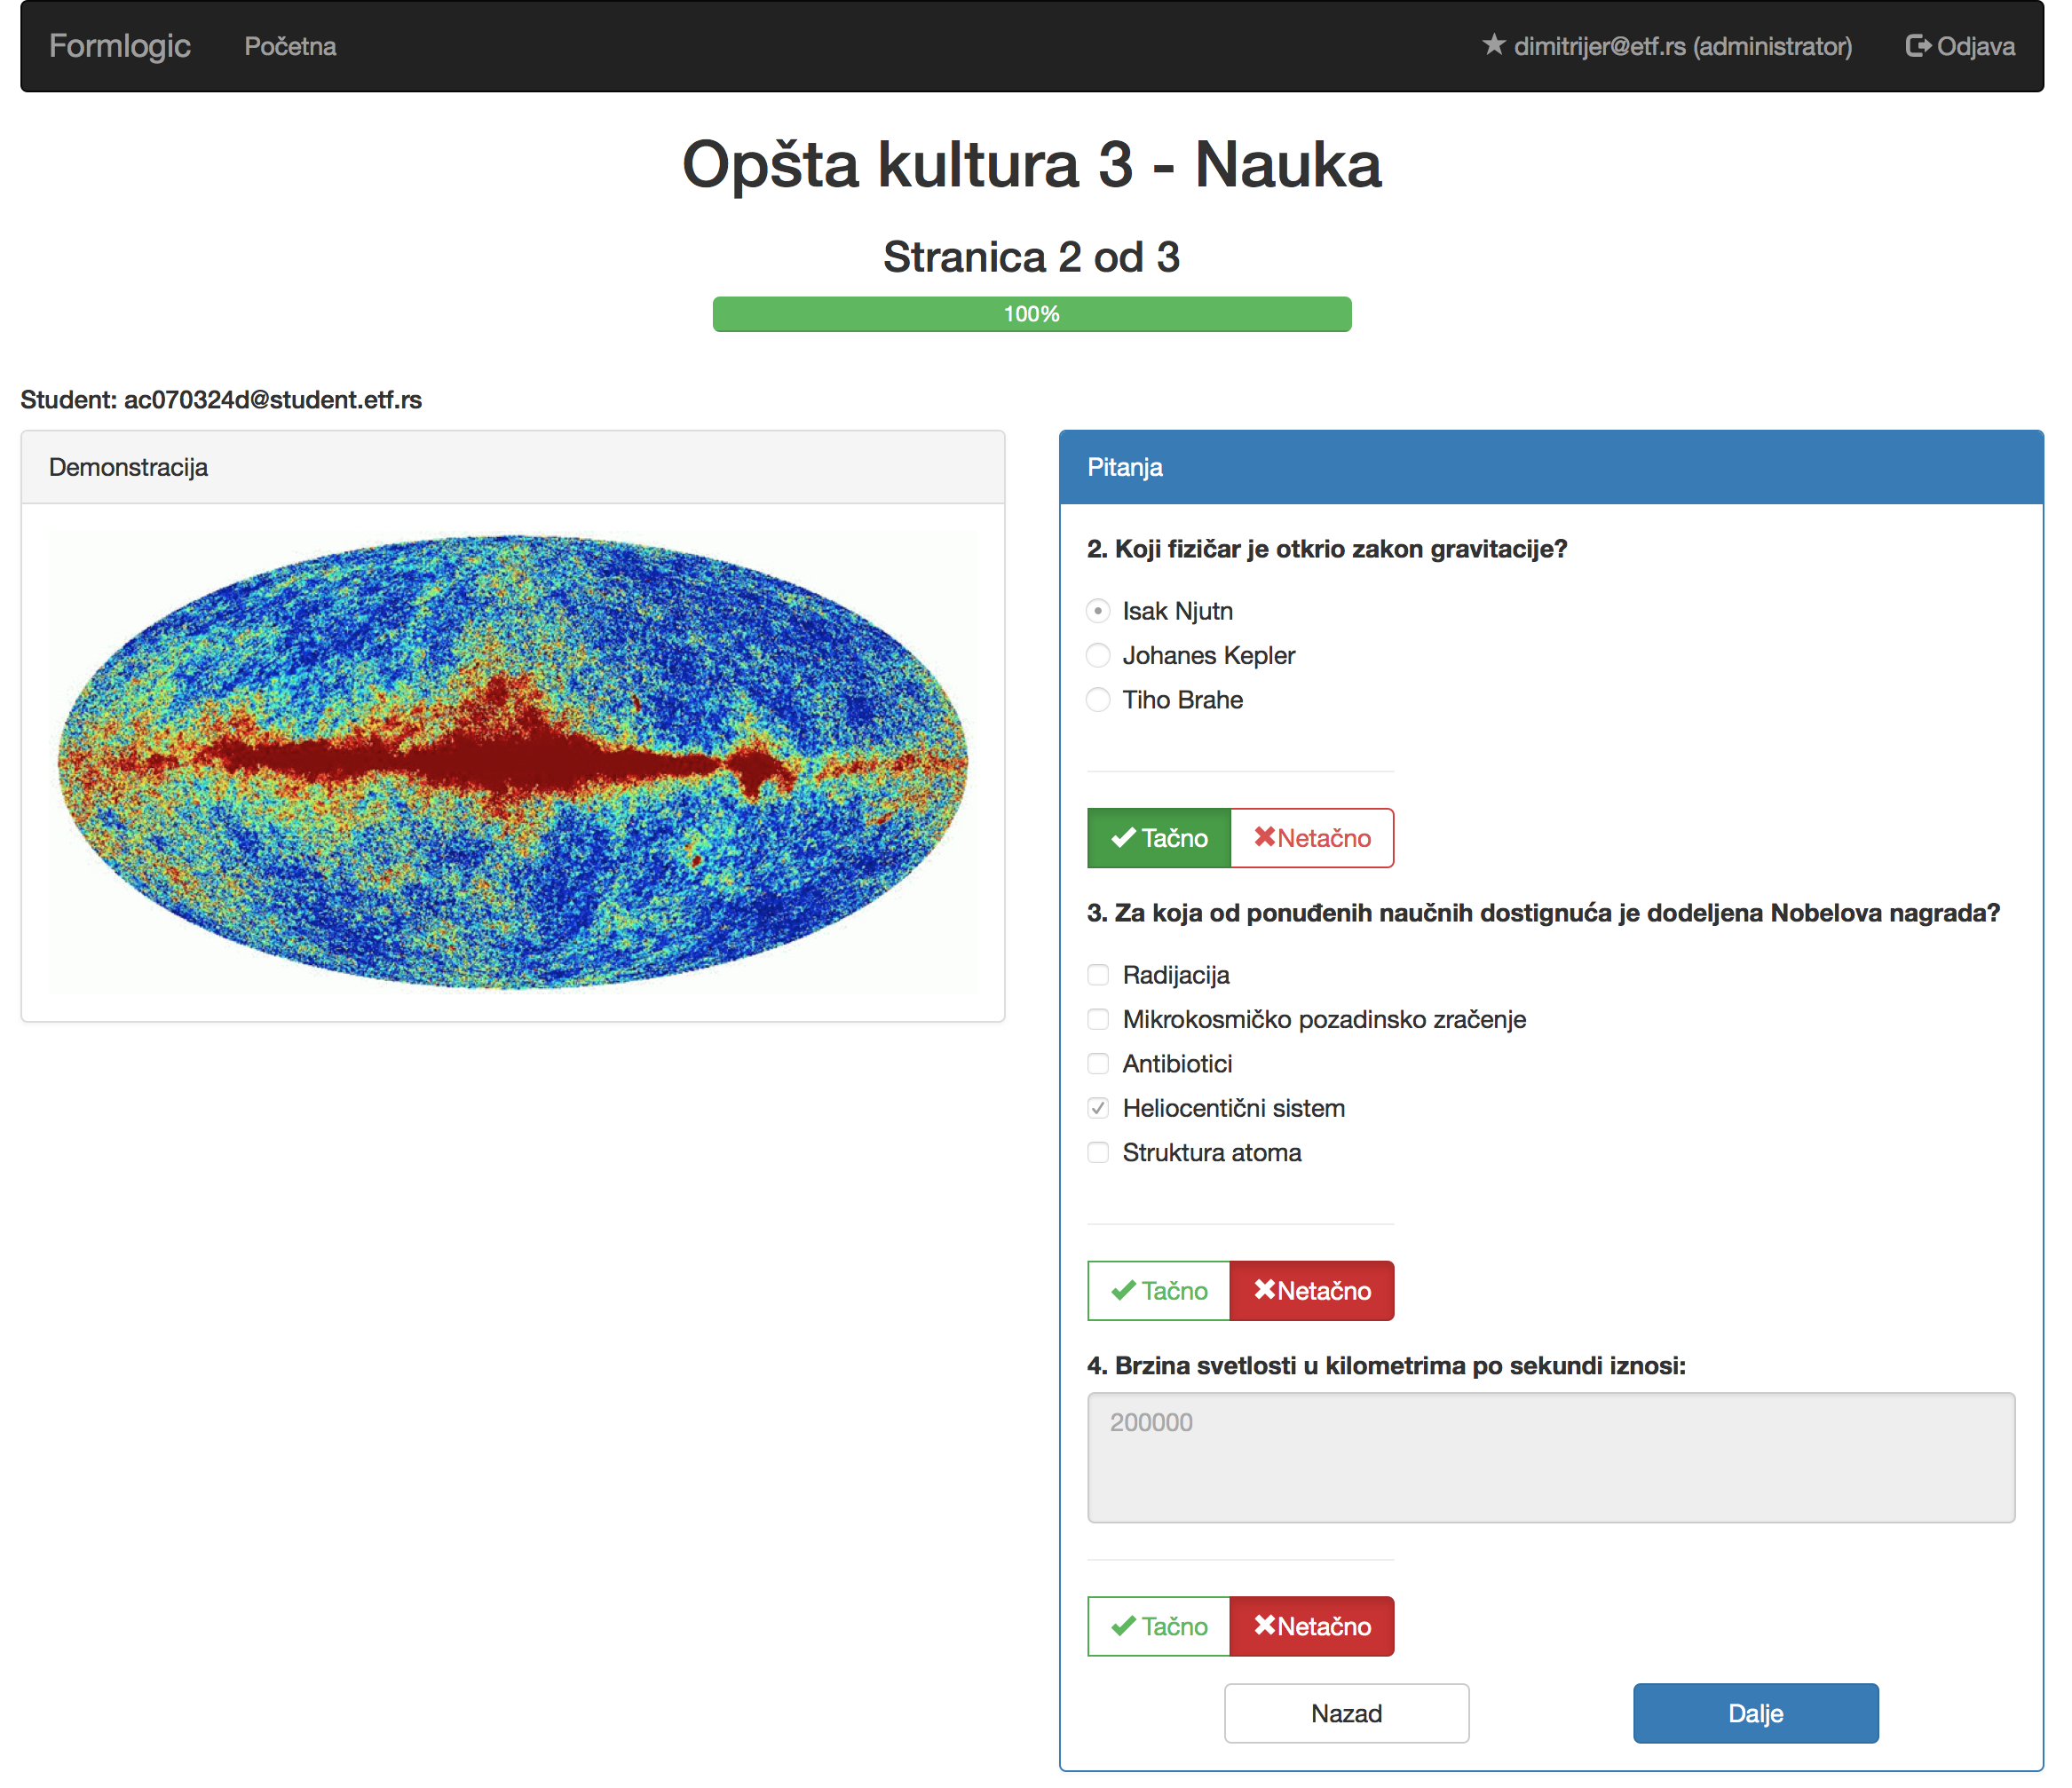
\includegraphics[width=0.75\textwidth]{task-admin}}
\end{frame}

\section{Realizacija sistema}
\begin{frame}[fragile]
\frametitle{Izazovi tokom realizacije}
\begin{itemize}
\item Uprošćavanje stabla parsiranja
\item Prilagođene 404 i 500 stranice
\item Dohvatanje testova sa ocenama unutar jednog SQL upita
\item Raspakivanje \texttt{Jdbc4Array} nizova unutar transakcije
\item Slanje \textit{anti-forgery} tokena sa POST zahtevima
\end{itemize}
\centering
\begin{Verbatim}[framesep=2mm,labelposition=bottomline,frame=single,label=Primer stabla parsiranja,fontsize=\tiny]
[:QuantifiedFormula
 [:Quantifier [:FOREACH] [:LITERAL "x"]]
 [:Implication
  [:Conjunction [:Negation [:LITERAL "x"]] [:LITERAL "y"]]
  [:Predicate [:PRED "Inv"] [:LITERAL "y"] [:LITERAL "x"]]]]
\end{Verbatim}
\begin{center}
\fbox{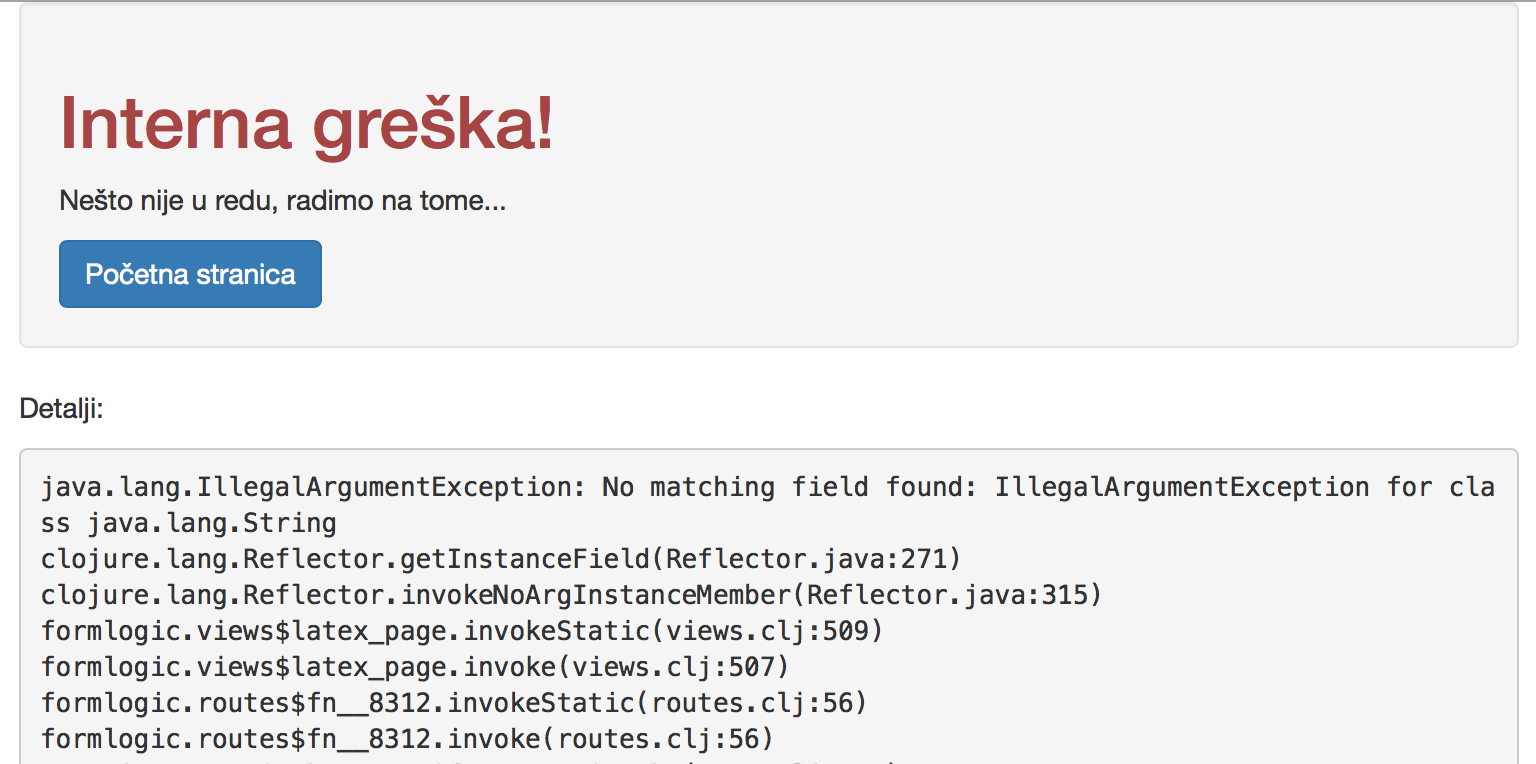
\includegraphics[width=0.4\textwidth]{500}}
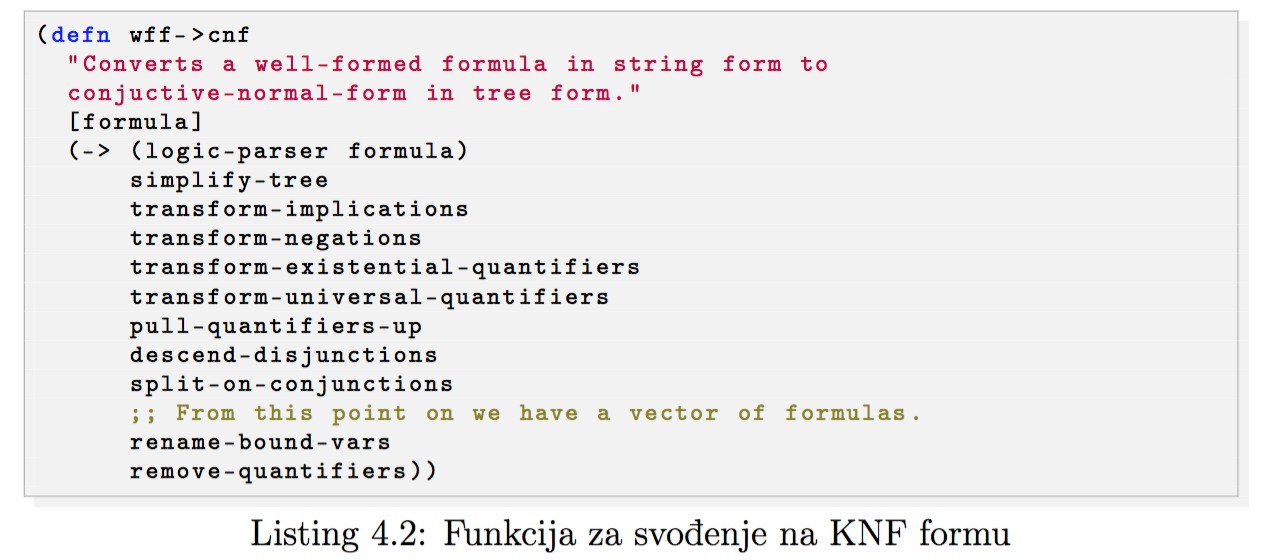
\includegraphics[width=0.45\textwidth]{wff-screenshot}
\end{center}
\end{frame}

\begin{frame}
\frametitle{Moguća unapređenja}
\begin{itemize}
\item UI za unos testova
\item Vremenko ograničenje za izradu testa
\item Grupe studenata
\item SSL
\item Skalarno ocenjivanje odgovora
\item Paginacija rezultata pretrage
\item ...
\end{itemize}
\end{frame}

\section{Zaključak}
\begin{frame}
\frametitle{Zaključak}
Realizovan je funckionalan sistem koji je:
\begin{itemize}
\item lagan (< 2000 LOC)
\item modularan
\item pogodan za distribuciju
\item otvorenog koda: \url{https://github.com/dimitrijer/formlogic}
\end{itemize}
Clojure kao jezik:
\begin{itemize}
\item potrebno neko vreme za navikavanje
\item nema stanja, samo vrednosti
\item kombinovanje f-ja veoma moćno
\item nije ,,isključivo'' funkcionalni jezik
\end{itemize}
\end{frame}

\begin{frame}
\centering
\Large \bfseries Hvala na pažnji!
\end{frame}
\end{document}